%%%% compile with
%%% latexmk -auxdir=aux/ main.tex
\documentclass{irdbeamer}
\usepackage{tikz}
\usepackage{pgfplots}
\usepackage{animate}
% \usepackage{listings}
% \usepackage{minted}

\title{Projections and clusterings}
\subtitle{AI for ecologists}
\author[Paul Tresson]{Paul Tresson}
\date{21/05/25} % or whatever the date you are presenting in is
% \institute[Institut de Recherche pour le Développement]{UMR AMAP}

%\copyrightnotice{Published by Institut de Recherche pour le Développement, with permission}

% %% to add a background image for the title slide, uncomment here
% \usebackgroundtemplate{
%   \tikz[overlay, remember picture] \node[at=(current page.center)] {
%     \includegraphics[width=\paperwidth,height=\paperheight]{example-image-a}
%   };
% }
\definecolor{C0}{rgb}{0.0,0.3,0.6}
\definecolor{A0}{rgb}{1.0,0.0,0.0}
\definecolor{B0}{rgb}{1.0,0.4,0.0}
\definecolor{A1}{rgb}{1.0,0.1,0.0}
\definecolor{C1}{rgb}{0.4,0.6,0.3}
\definecolor{C2}{rgb}{0.2,0.4,0.4}

\def\tdist{%
    gamma(.5*(1+1))/(sqrt(1*pi)*gamma(.5*1))*((1+x^2/1)^(-.5*(1+1)))%
    % gamma(.5*(\n+1))/(sqrt(\n*pi)*gamma(.5*\n))*((1+x^2/\n)^(-.5*(\n+1)))%
}

\usepackage[
    backend=biber,
    style=authoryear-comp,
    maxcitenames=2, % max 2 authors before switching to et al.
    maxbibnames=4,
    uniquelist=false, % stays et al. when almost the same authors
    uniquename=false, % dose not bother when first name not written the same way everywhere
    date=year, % month does not appear in bibliography
    natbib=true, % use natbib synthax
    url=false, % remove url
    eprint=false % remove eprint
]{biblatex}

\addbibresource{refs.bib}

% % Define the color for citations
% \definecolor{citecolor}{gray}{0.5} % 0.5 is the gray level, adjust as needed

% % Redefine citation commands to include the color
% \renewcommand{\cite}[1]{\textcolor{citecolor}{\citet{#1}}}
% \renewcommand{\citep}[1]{\textcolor{citecolor}{\citep{#1}}}
% \renewcommand{\citet}[1]{\textcolor{citecolor}{\citet{#1}}}

\let\oldcite=\cite                                                              
\renewcommand{\cite}[1]{\textcolor[rgb]{.5,.5,.7}{\oldcite{#1}}}
\let\oldcitep=\citep                                                              
\renewcommand{\citep}[1]{\textcolor[rgb]{.5,.5,.7}{\oldcitep{#1}}}

\begin{document}

\addlogo{logos/IRD_banner.png}
\addlogo{logos/AMAP_banner.png}
\addlogo{logos/CESAB.jpg}
\maketitle

\usebackgroundtemplate{}

\section{Introduction}

\begin{frame}{Visualize what is happening in higher dimensions}
    \centering
    \begin{tabular}{ccc}
        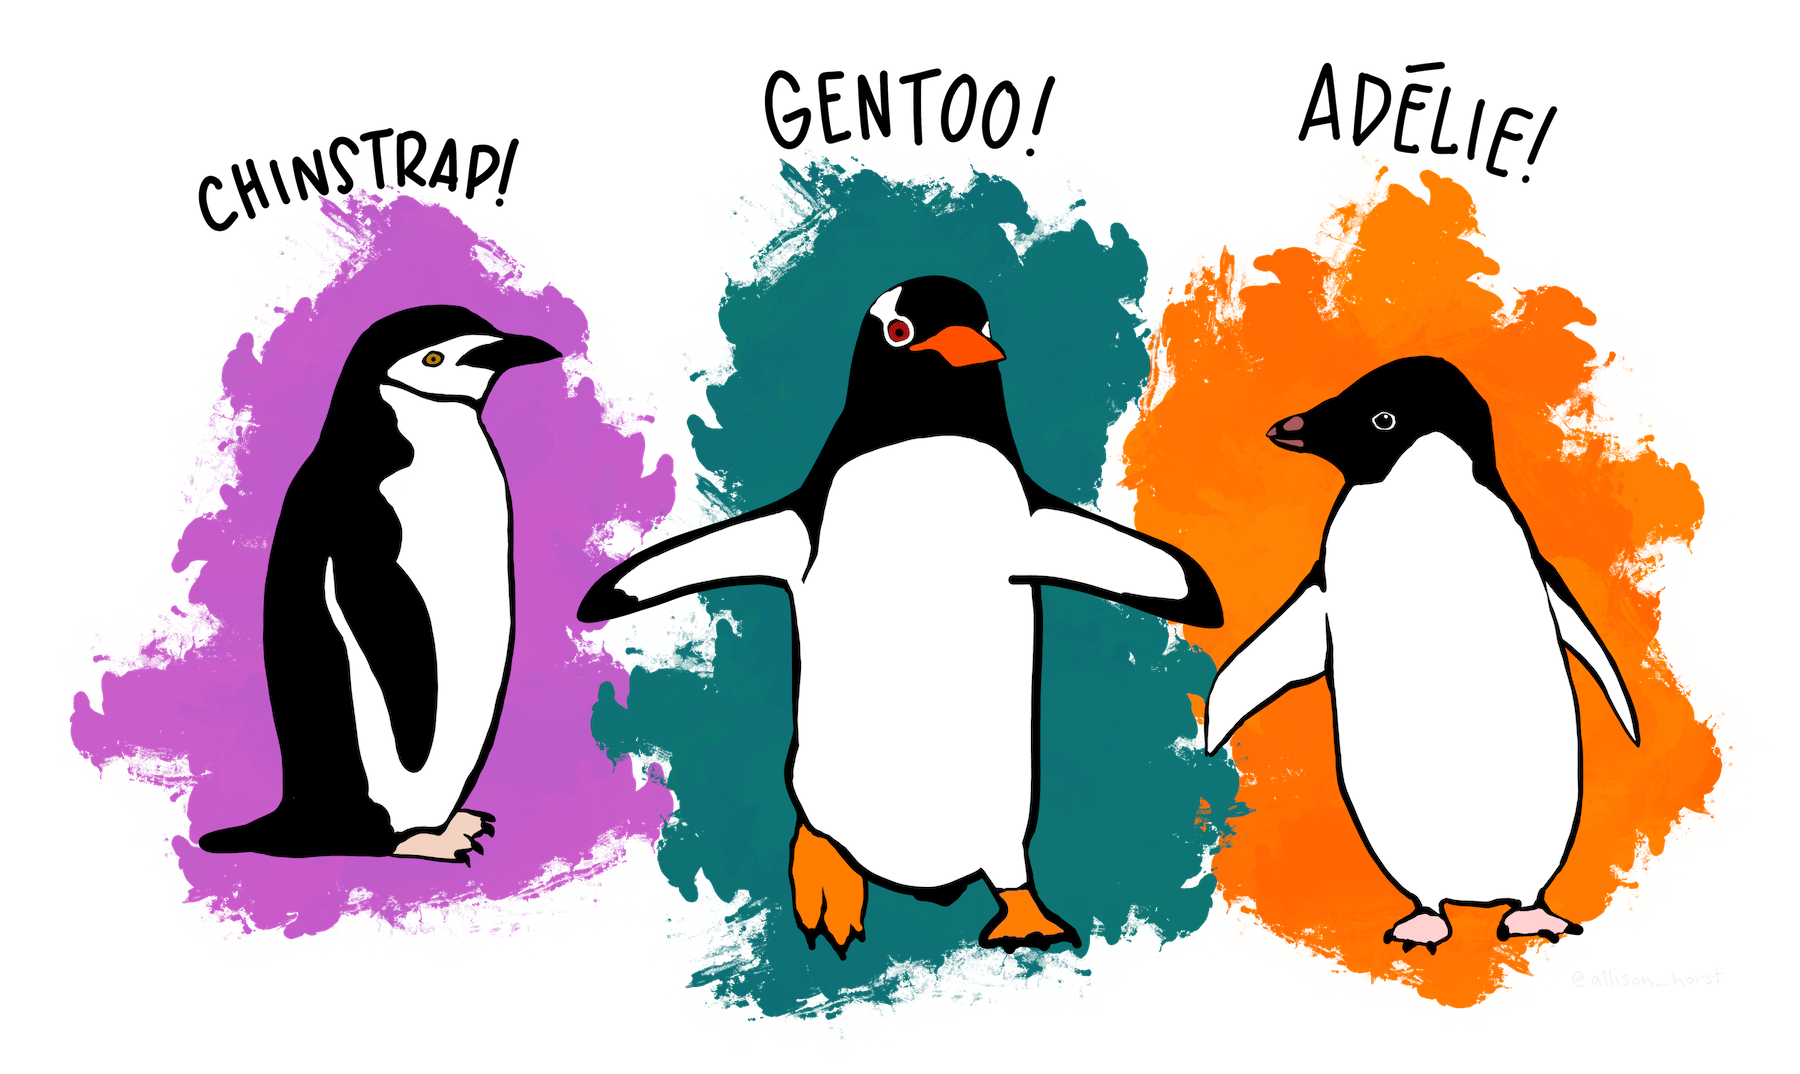
\includegraphics[width=0.2\textwidth]{./figs/lter_penguins.png}&
        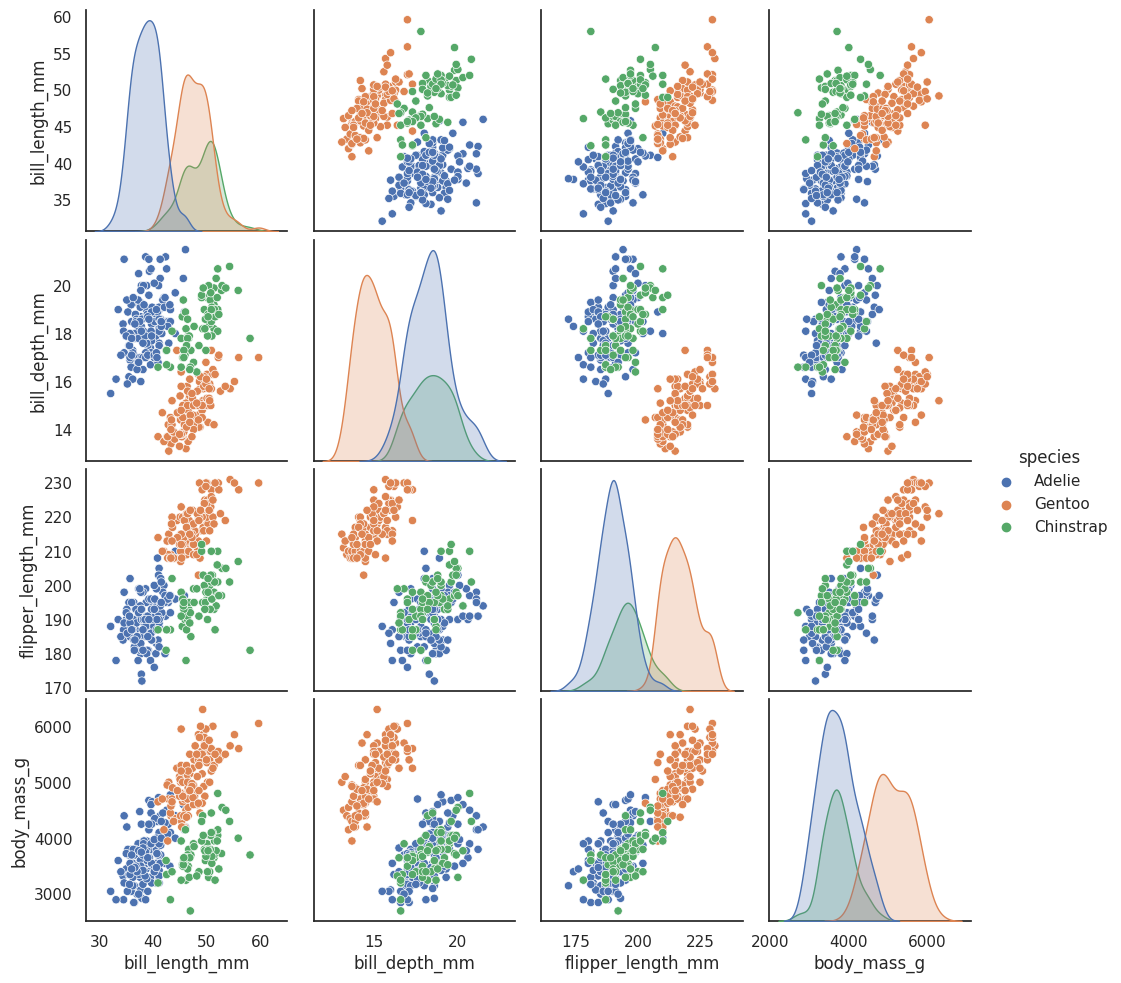
\includegraphics[width=0.5\textwidth]{./figs/penguins.png}&
        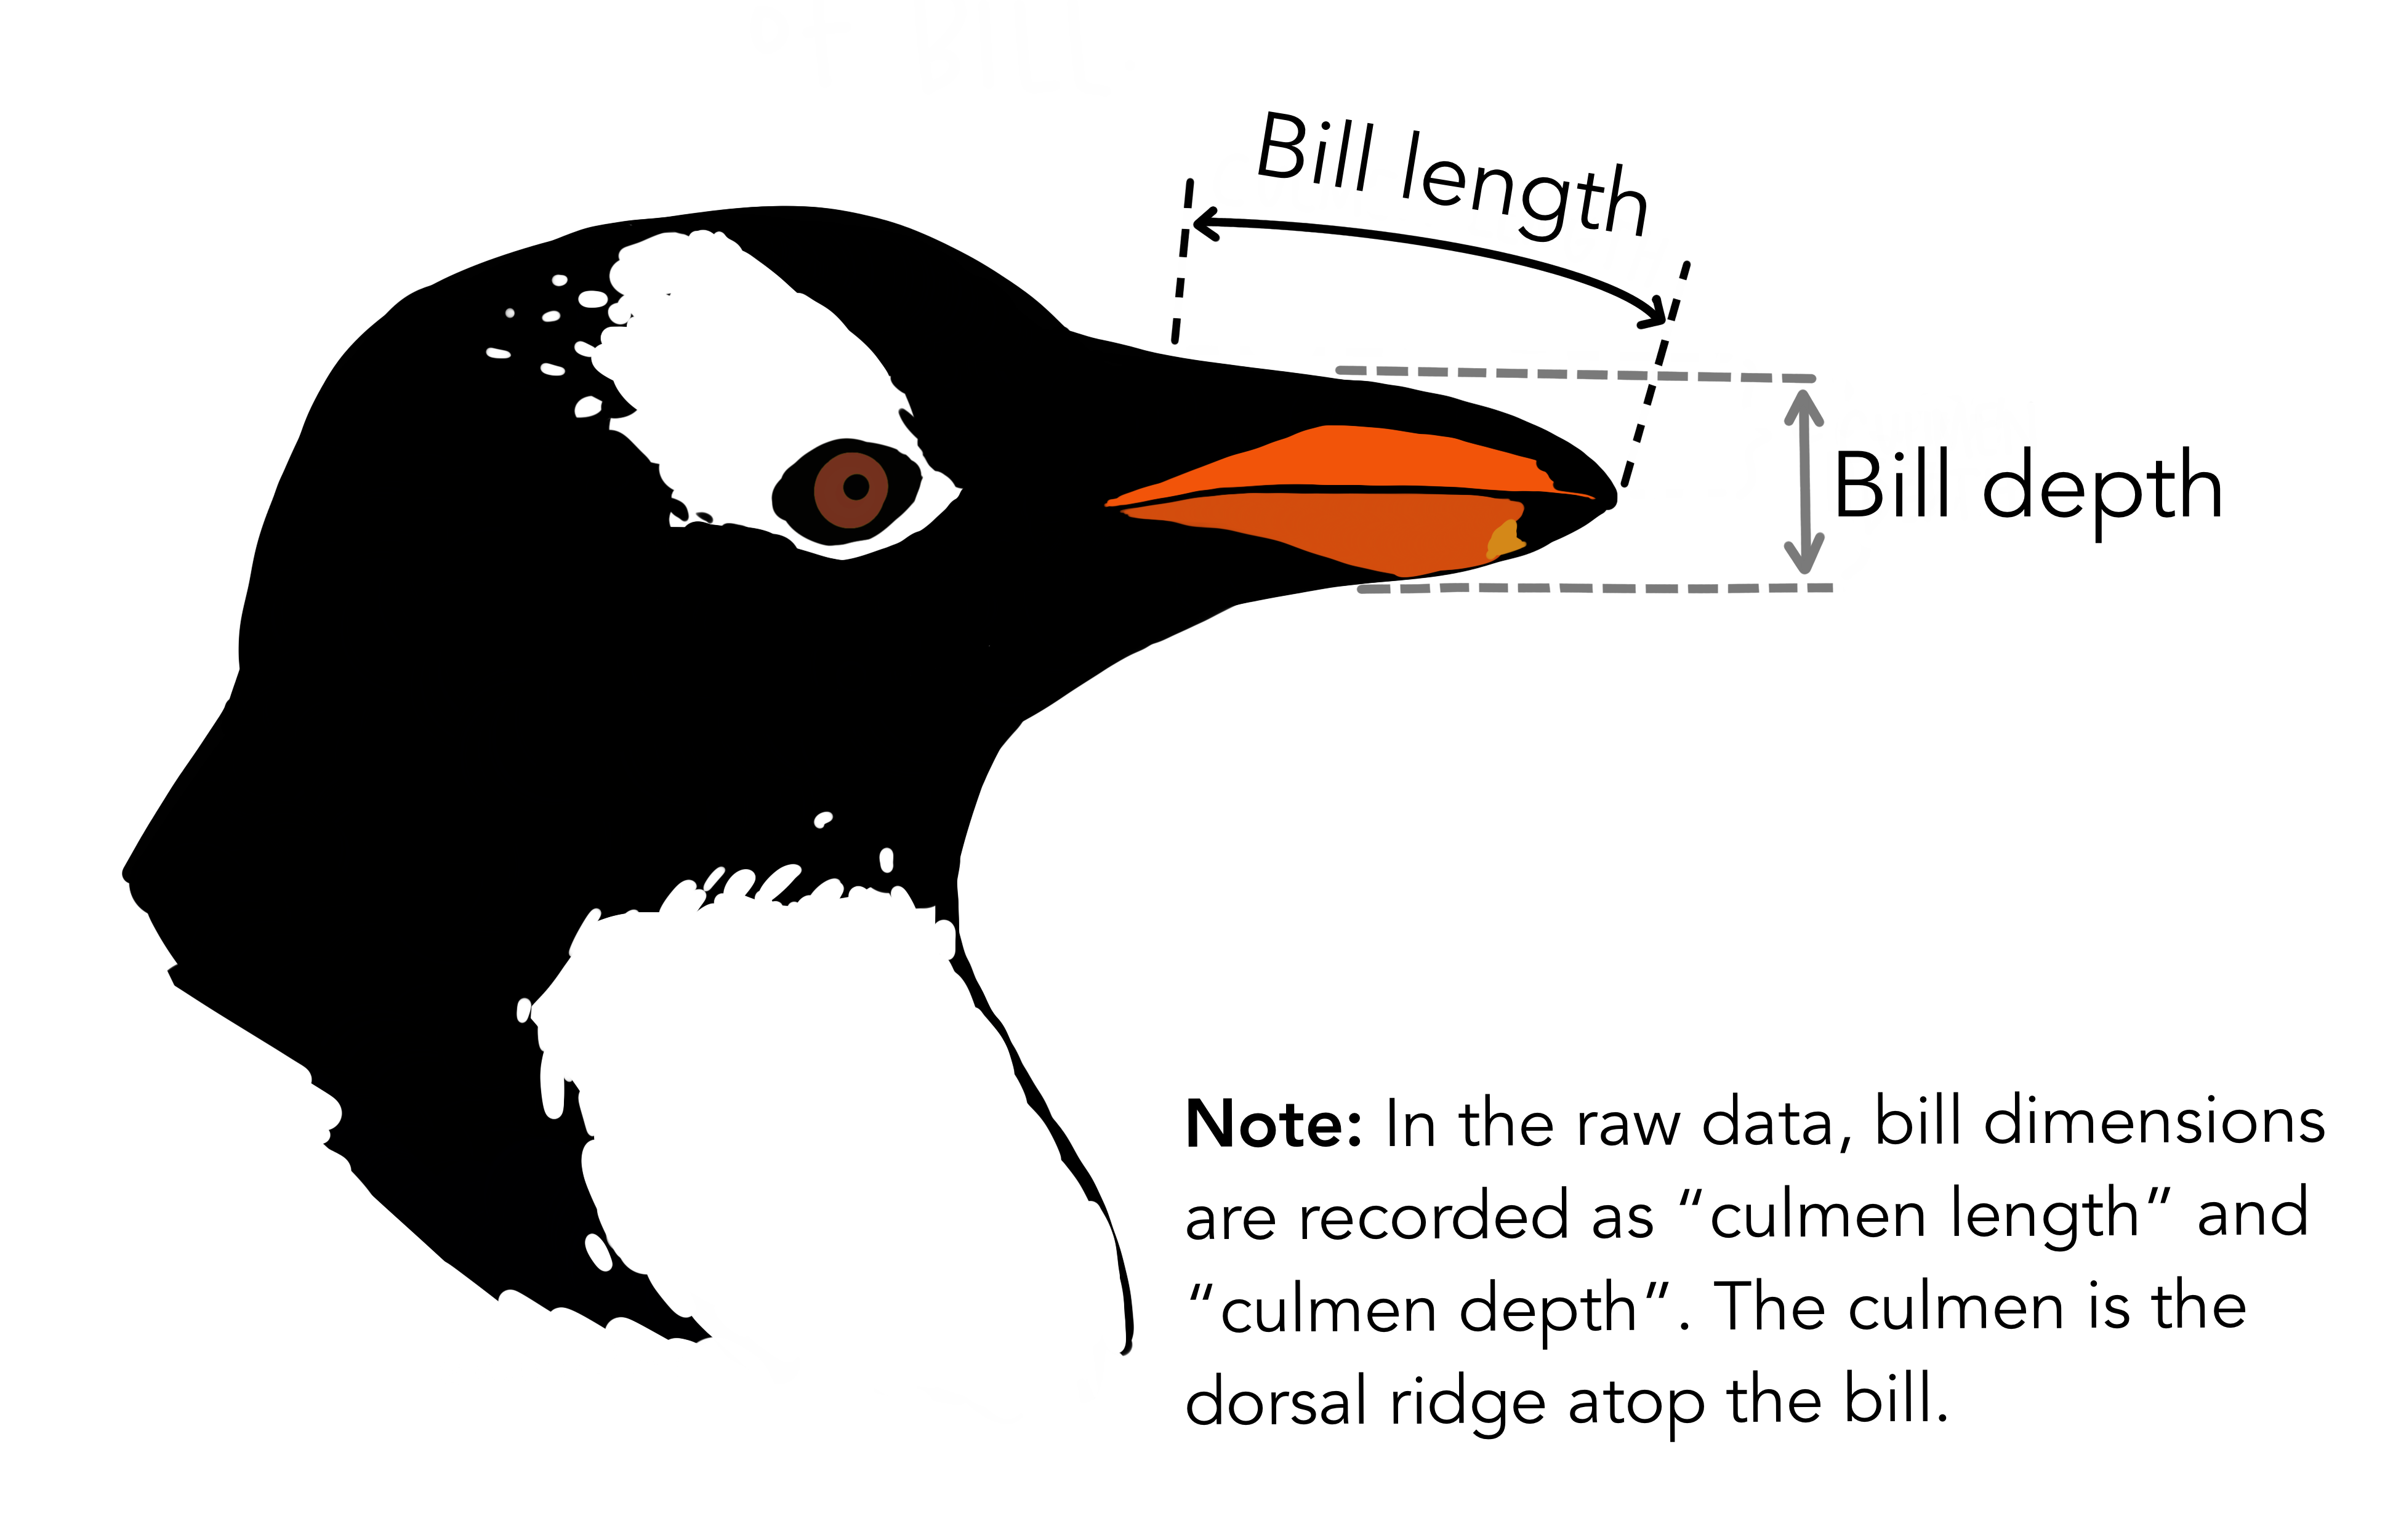
\includegraphics[width=0.2\textwidth]{./figs/culmen_depth.png}\\
    \end{tabular}
\end{frame}

\begin{frame}{Visualize what is happening in higher dimensions}
    \centering
        \includegraphics<1>[width=0.5\textwidth]{./figs/mnist.png}%
        \includegraphics<2>[width=0.5\textwidth]{./figs/mnist_pairplot.png}%
        \includegraphics<3>[width=0.5\textwidth]{./figs/mnist_umap.png}%
\end{frame}



\section{Projections}
\subsection{PCA}

\begin{frame}{PCA}
    \centering
        \includegraphics<1>[width=0.5\textwidth]{./figs/pca1.png}%
        \includegraphics<2>[width=0.5\textwidth]{./figs/pca2.png}%
\end{frame}

\begin{frame}{PCA calculation}
    \scriptsize
    \begin{columns}
\begin{column}{0.25\textwidth}
    \only<1->{
    $$X = \begin{bmatrix} x_1 & y_1 \\ x_2 & y_2 \\ x_3 & y_3 \\ ... & ... \end{bmatrix}$$
    }
\end{column}
\begin{column}{0.25\textwidth}
    \only<2->{
   $$C = \frac{1}{n-1}X^TX$$ 
   $$C = \begin{bmatrix} \sigma_{x}^2 & \sigma_{xy} \\ \sigma_{yx} & \sigma_{y}^2 \end{bmatrix}$$ 
    }
\end{column}
\begin{column}{0.25\textwidth}
    \only<3->{
   $$Cv = \lambda v$$ 
   $$\begin{bmatrix} \sigma_{x}^2 & \sigma_{xy} \\ \sigma_{yx} & \sigma_{y}^2 \end{bmatrix} \begin{bmatrix} v_x \\ v_y \end{bmatrix} = \lambda \begin{bmatrix} v_x \\ v_y \end{bmatrix}$$
    }
\end{column}
\begin{column}{0.25\textwidth}
    \only<4->{
   $$P = \begin{bmatrix} v_x & v_y \end{bmatrix}$$ 
    }
\end{column}
\end{columns}
\end{frame}

\begin{frame}{PCA calculation}
\centering
    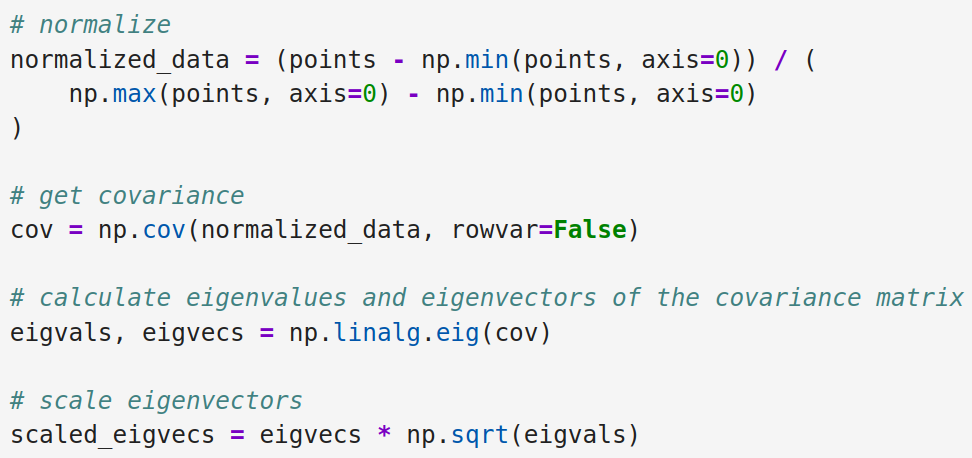
\includegraphics[width=.8\textwidth]{./figs/pca_numpy.png}
\end{frame}

% \begin{frame}{PCA calculation}
%    $$C = \begin{bmatrix} \sigma_{x}^2 & \sigma_{xy} \\ \sigma_{yx} & \sigma_{y}^2 \end{bmatrix}$$ 
% \end{frame}

% \begin{frame}{PCA calculation}
%    $$Cv = \lambda v$$ 
%    $$\begin{bmatrix} \sigma_{x}^2 & \sigma_{xy} \\ \sigma_{yx} & \sigma_{y}^2 \end{bmatrix} \begin{bmatrix} v_x \\ v_y \end{bmatrix} = \lambda \begin{bmatrix} v_x \\ v_y \end{bmatrix}$$
% \end{frame}

% \begin{frame}{PCA calculation}
%    $$P = \begin{bmatrix} v_x & v_y \end{bmatrix}$$ 
% \end{frame}

% \begin{frame}[fragile]{PCA}
%     % \begin{lstlisting}[language=Python]
% % normalized_data = (points - np.min(points, axis=0)) / (
%     % np.max(points, axis=0) - np.min(points, axis=0)
% % )
% % mean = np.mean(normalized_data, axis=0)
% % cov = np.cov(normalized_data, rowvar=False)

% % # Calculate eigenvalues and eigenvectors of the covariance matrix
% % eigvals, eigvecs = np.linalg.eig(cov)

% % # Scale eigenvectors
% % scaled_eigvecs = eigvecs * np.sqrt(eigvals)
%     % \end{lstlisting}

%     \rule{\textwidth}{1pt}
% \scriptsize
% \begin{minted}{python}
%     # This program adds two numbers
%     num1 = 1.5
%     num2 = 6.3
%     # Add two numbers
%     sum = num1 + num2
%     # Display the sum
%     print('The sum of {0} and {1} is {2}'.format(num1, num2, sum))
% \end{minted}
% \rule{\textwidth}{1pt}
% \end{frame}

% \begin{frame}{PCA}
%     \centering
%         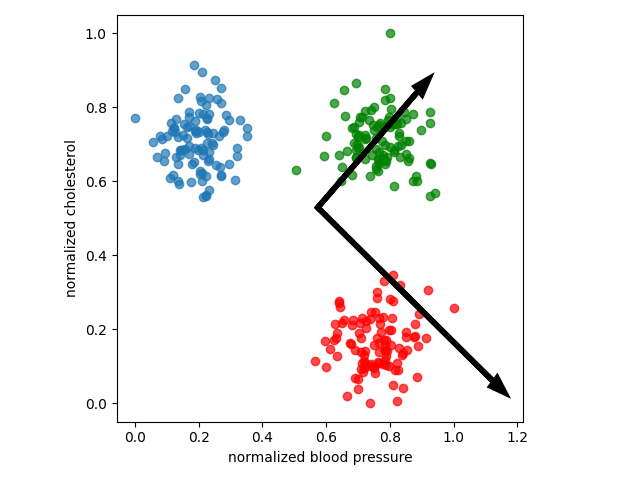
\includegraphics[width=0.5\textwidth]{./figs/pca3.png}%
% \end{frame}



\begin{frame}{PCA advantages and drawbacks}
\begin{columns}
\begin{column}{0.05\textwidth}
\begin{itemize}
    \item[] 
    \item[] 
    \item[] 
\end{itemize}
\end{column}
    \column{0.45\linewidth}
        \textbf{Advantages}
        \begin{itemize}
            \item<1-> fast
            \item<2-> scales well
            \item<3-> explainatory
        \end{itemize}
    \column{0.45\linewidth}
        \textbf{Drawbacks}
        \begin{itemize}
            \item<4-> \textbf{not suited for non-linear data}
            \item[] 
            \item[] 
        \end{itemize}
\end{columns}
\end{frame}

\begin{frame}{Non linear data}
    \begin{figure}
    \centering
    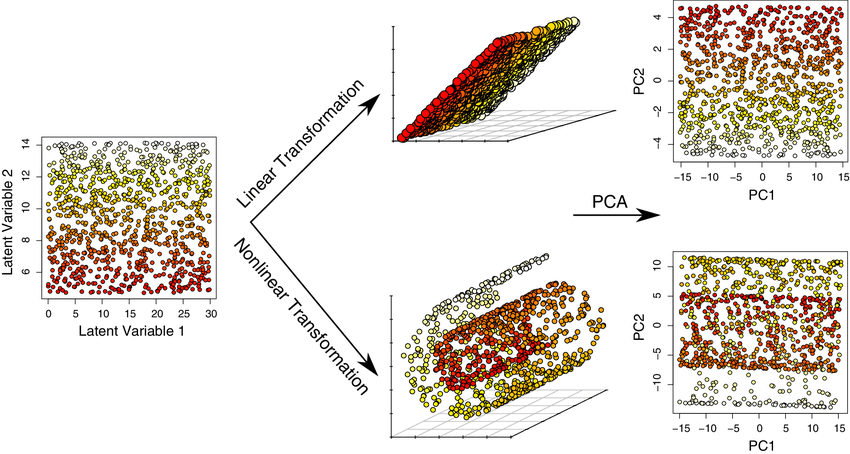
\includegraphics[width=.7\textwidth]{./figs/non_linearity.png}
    \caption{\tiny Figure from \cite{du2019dimensionality}}
    \end{figure}
\end{frame}

\subsection{UMAP}

\begin{frame}{How to work with non linear data}
    \begin{enumerate}
        \item Find a good representation of the data in high dimension
        \item Fit a good representation of in low dimension
    \end{enumerate}
\end{frame}

\begin{frame}{Classics}
    \begin{itemize}
        \item<1->\textbf{SNE} (Stochastic Neighbor Embedding) \cite{hinton2002stochastic}
        \item<2->\textbf{T-SNE} (T-distributed SNE) \cite{van2008visualizing}
        \item<3->\textbf{UMAP} (Uniform Manifold Approximation and Projection) \cite{mcinnes2018umap}
    \end{itemize}
\end{frame}

\begin{frame}{UMAP : Finding high dimension graph}
\begin{columns}
\begin{column}{0.5\textwidth}
\centering
    \includegraphics<1>[width=\textwidth]{./figs/umap/1_all_points.png}%
    \includegraphics<2>[width=\textwidth]{./figs/umap/2_sampled.png}%
    \includegraphics<3>[width=\textwidth]{./figs/umap/3_knn.png}%
\end{column}
\begin{column}{0.5\textwidth}
\end{column}
\end{columns}
\end{frame}

\begin{frame}{UMAP : Fitting low dimensional representation}
\begin{columns}
    \begin{column}[t]{0.5\textwidth}
\centering
    \includegraphics<1>[width=\textwidth]{./figs/umap/3_knn.png}%
    \includegraphics<2>[width=\textwidth]{./figs/umap/4-1_opti.png}%
    \includegraphics<3>[width=\textwidth]{./figs/umap/4-2_opti.png}%
    \includegraphics<4->[width=\textwidth]{./figs/umap/4-3_opti.png}%
\end{column}
    \begin{column}[t]{0.5\textwidth}
\centering
    \includegraphics<1-4>[width=\textwidth]{./figs/umap/4-1_spectral.png}%
    \includegraphics<5>[width=\textwidth]{./figs/umap/4-2_spectral.png}%
    \includegraphics<6>[width=\textwidth]{./figs/umap/4-3_spectral.png}%
    \includegraphics<7->[width=\textwidth]{./figs/umap/4-4_spectral.png}%
\end{column}
\end{columns}
\end{frame}

\begin{frame}{Mammoth example}
    \centering
    \vspace{-.5cm}
    \includegraphics<1>[width=.6\textwidth]{./figs/mammoth/3d_single.png}%
    \includegraphics<2>[width=.6\textwidth]{./figs/mammoth/3d_color.png}%
\end{frame}

\begin{frame}{Mammoth example - PCA}
    \centering
    \vspace{-.5cm}
    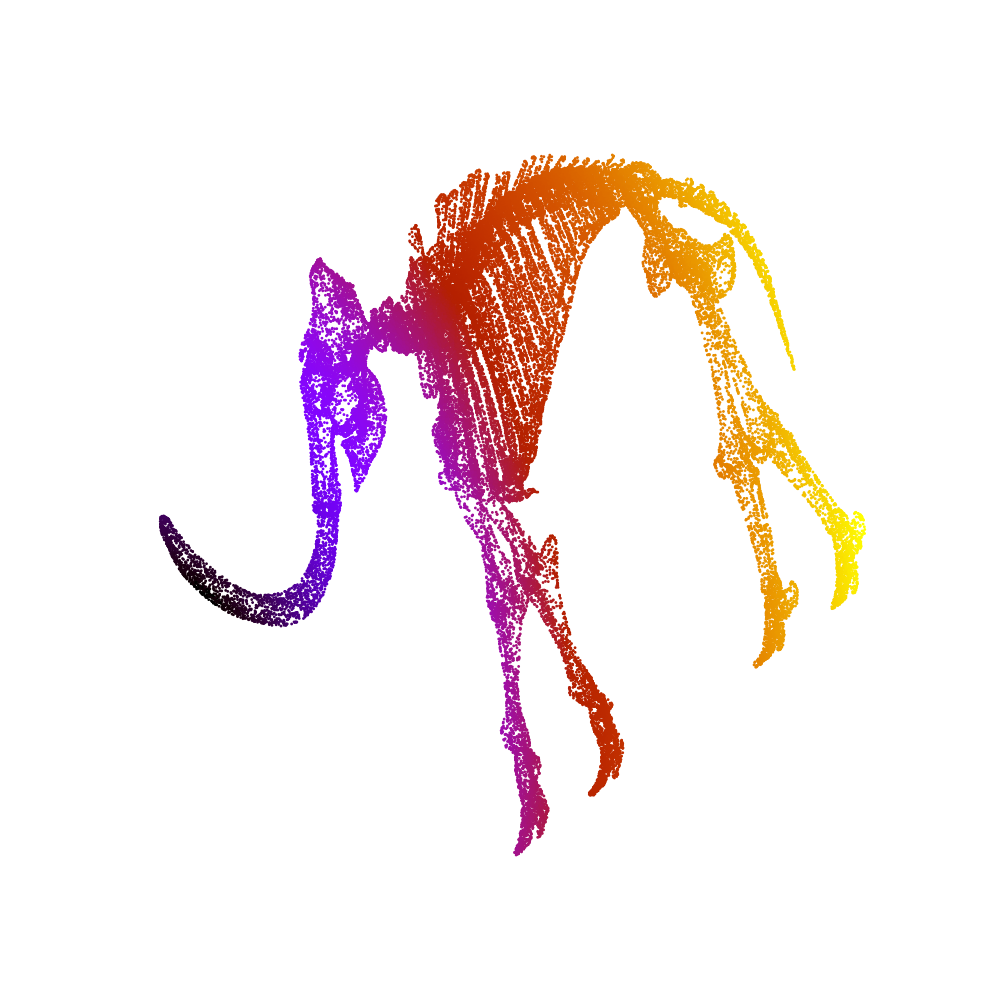
\includegraphics[width=.6\textwidth]{./figs/mammoth/pca.png}
\end{frame}

\begin{frame}{Mammoth example - UMAP}
    \centering
    \vspace{-.5cm}
    \includegraphics<1>[width=.6\textwidth]{./figs/mammoth/n5.png}%
    \includegraphics<2>[width=.6\textwidth]{./figs/mammoth/n7.png}%
    \includegraphics<3>[width=.6\textwidth]{./figs/mammoth/n9.png}%
    \includegraphics<4>[width=.6\textwidth]{./figs/mammoth/n10.png}%
    \includegraphics<5>[width=.6\textwidth]{./figs/mammoth/n50.png}%
    \includegraphics<6>[width=.6\textwidth]{./figs/mammoth/n100.png}%
    \includegraphics<7>[width=.6\textwidth]{./figs/mammoth/n500.png}%
    \includegraphics<8>[width=.6\textwidth]{./figs/mammoth/n1000.png}%
\end{frame}

\begin{frame}{Mammoth example - Number of neighbors}
    \centering
    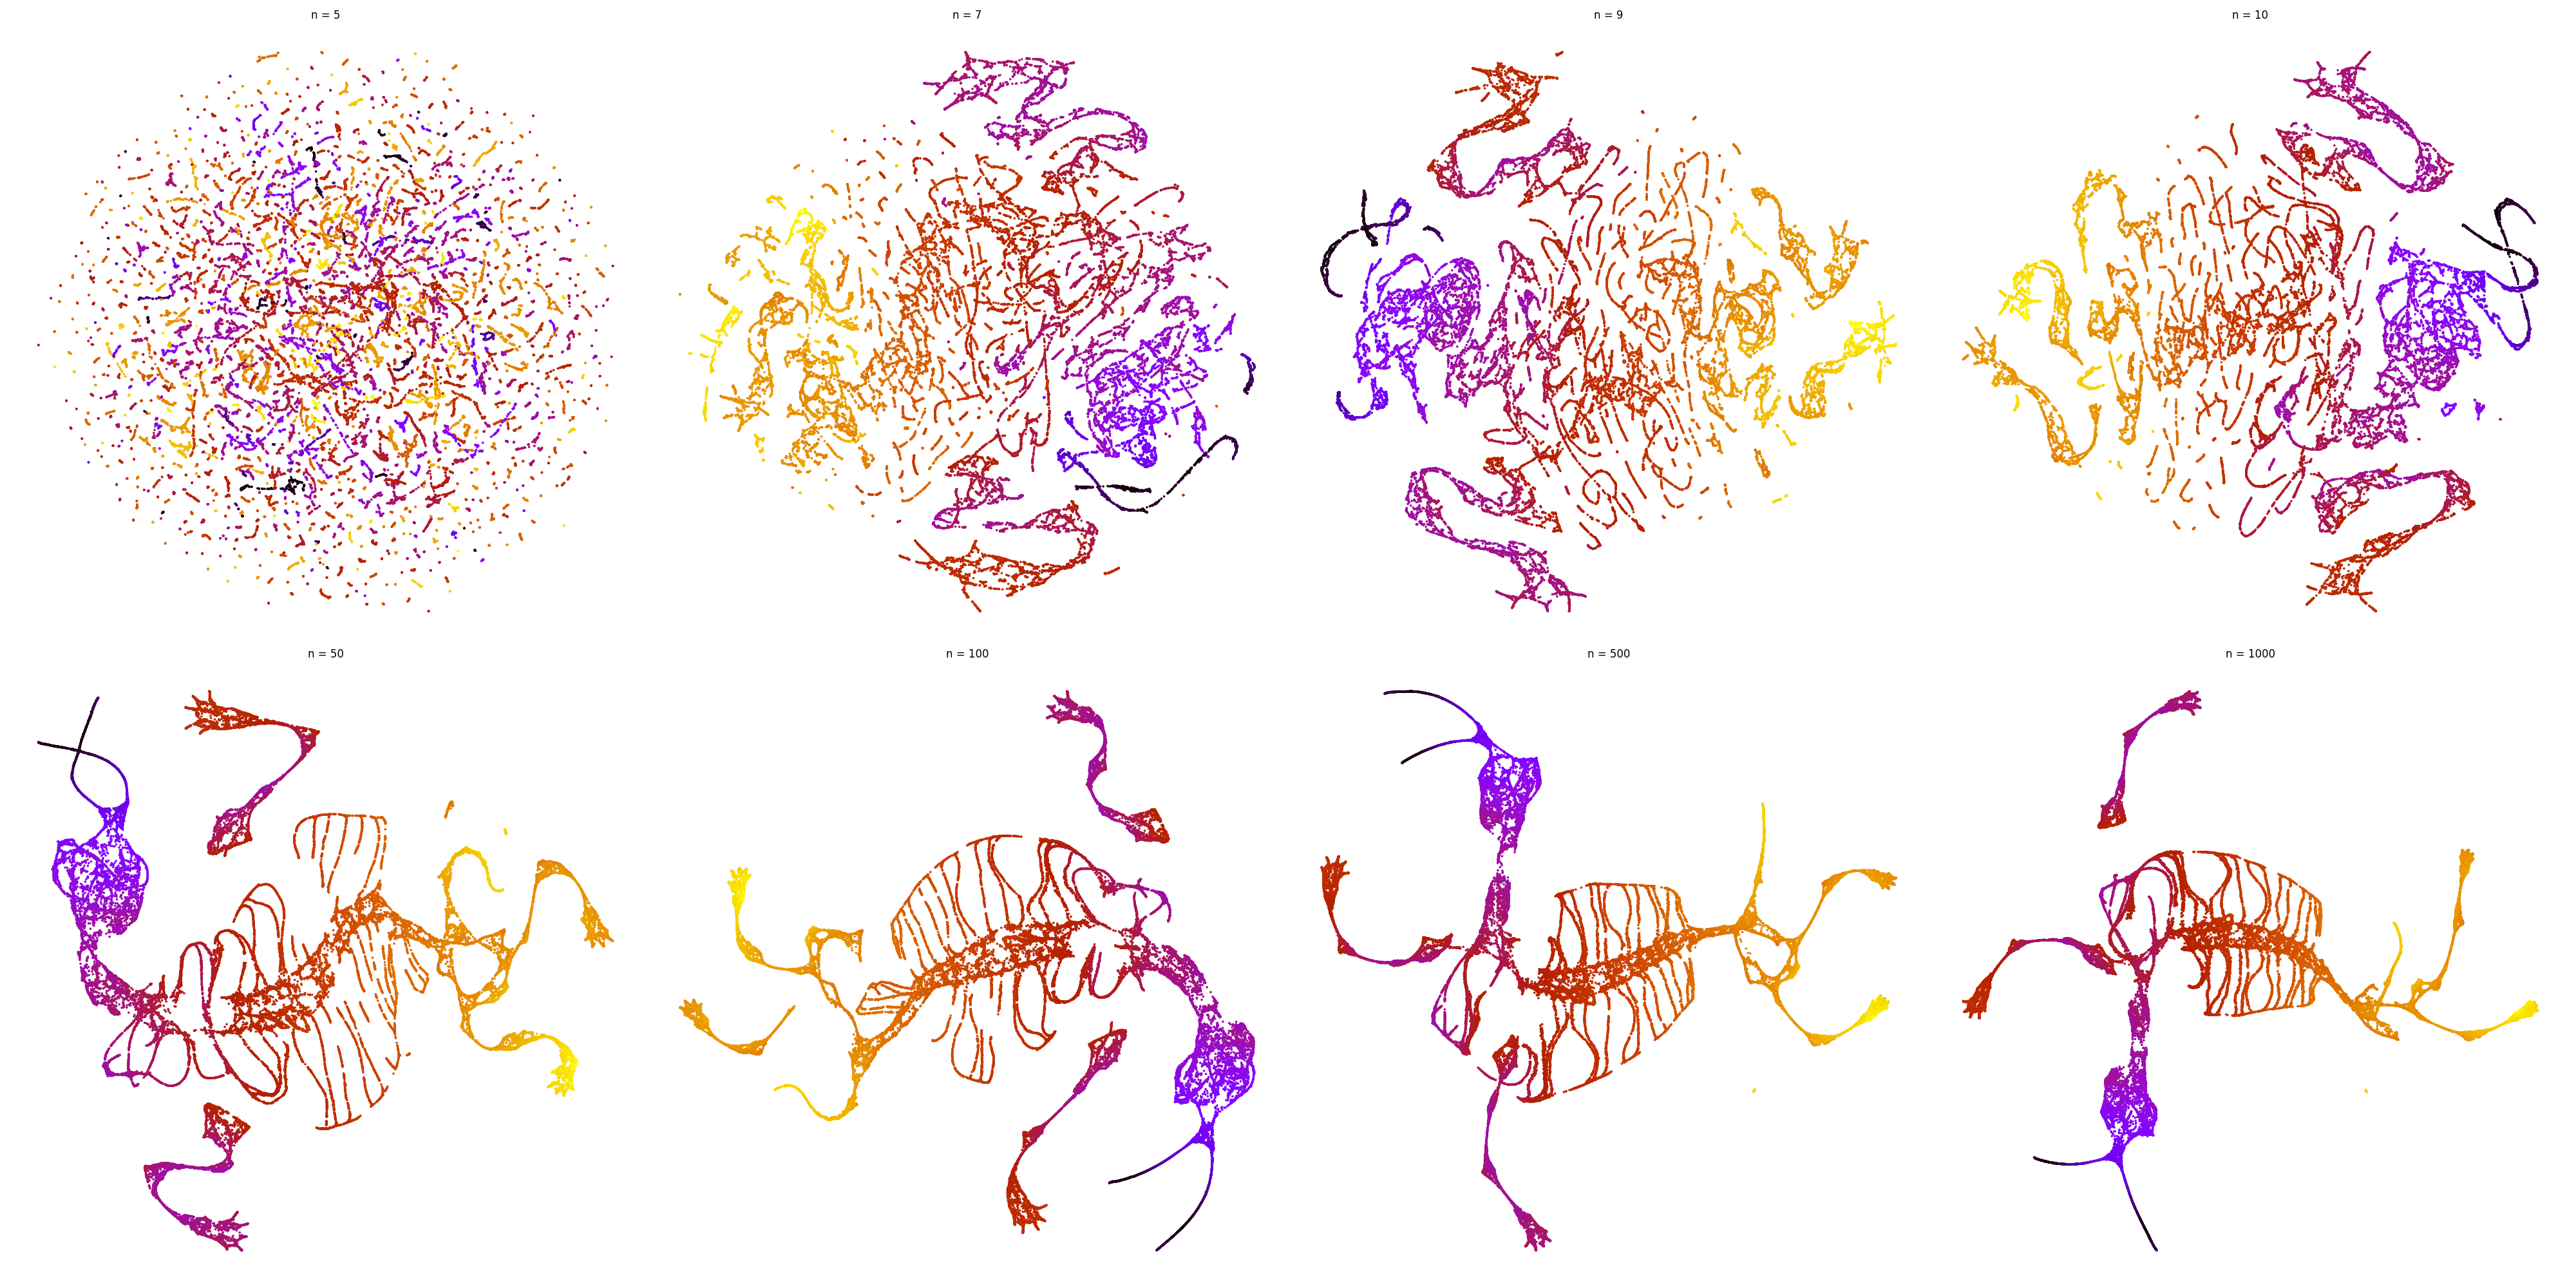
\includegraphics[width=.8\textwidth]{./figs/mammoth/combined_scatter_plots.png}
\end{frame}

\begin{frame}{UMAP vs. T-SNE}
\begin{columns}
\begin{column}{0.05\textwidth}
\begin{itemize}
    \item[] 
    \item[] 
    \item[] 
    \item[] 
    \item[] 
\end{itemize}
\end{column}
    \column{0.45\linewidth}
        \textbf{UMAP}
        \begin{itemize}
            \item<1-> graph theory, fuzzy logic
            \item<2-> determinist initialization
            \item<3-> $log_2$ similarity scores
            \item<4-> update by pairs 
            \item[$\rightarrow$]<4-> scales well for large datasets
        \end{itemize}
    \column{0.45\linewidth}
        \textbf{T-SNE}
        \begin{itemize}
            \item<1-> probabilities
            \item<2-> random initialization
            \item<3-> gaussian distribution similarity
            \item<4-> update all points
            \item[]<4-> scales less
        \end{itemize}
\end{columns}
\end{frame}

\begin{frame}{Scaling}
    \vspace{-.5cm}
    \begin{figure}
    \centering
    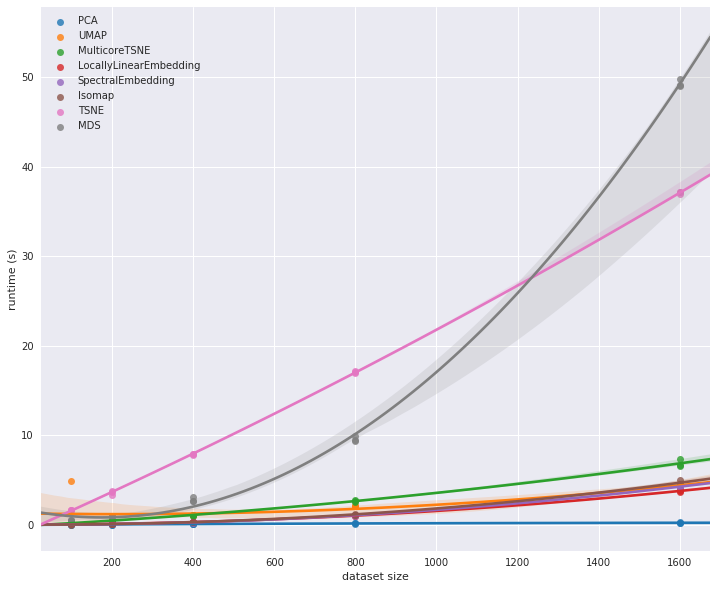
\includegraphics[width=.5\textwidth]{./figs/performance_umap.png}
    \caption{\tiny Figure from \href{https://umap-learn.readthedocs.io/en/latest/benchmarking.html}{umap-learn documentation}}
    \end{figure}
\end{frame}

% \begin{frame}{Animation}
%     %%% ffmpeg -i animation.gif -vsync 0 %04d.png
%     \centering
%   \animategraphics[autoplay,loop,controls,width=.7\linewidth]{20}{gif/}{0001}{0156}
%   % \animategraphics[loop,width=4cm]{10}{gif/}{0000}{0050}
% \end{frame}

\section{Clustering}

\subsection{K-means}
\begin{frame}{K-means}
    \centering
    \includegraphics<1>[width=.7\textwidth]{./figs/kmeans01.png}%
    \includegraphics<2>[width=.7\textwidth]{./figs/kmeans02.png}%
    \includegraphics<3>[width=.7\textwidth]{./figs/kmeans03.png}%
    \includegraphics<4>[width=.7\textwidth]{./figs/kmeans04.png}%
    \includegraphics<5>[width=.7\textwidth]{./figs/kmeans05.png}%
    \includegraphics<6>[width=.7\textwidth]{./figs/kmeans06.png}%
    \includegraphics<7>[width=.7\textwidth]{./figs/kmeans07.png}%
\end{frame}

\begin{frame}{Determine the good K ? Elbow method}
    \vspace{-.5cm}
    \begin{figure}
    \centering
    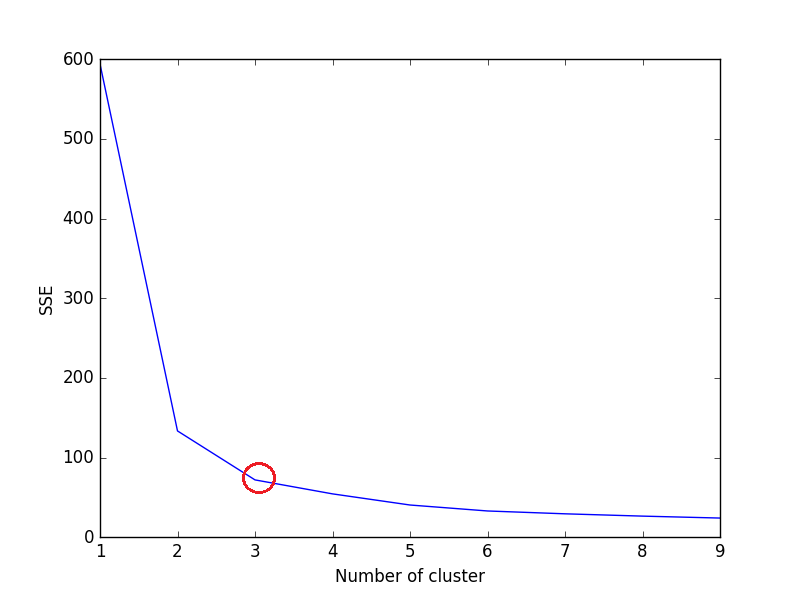
\includegraphics[width=.5\textwidth]{./figs/elbow.png}
    \caption{\tiny Figure from \href{https://stackoverflow.com/questions/19197715/scikit-learn-k-means-elbow-criterion}{SO}}
    \end{figure}
\end{frame}

\begin{frame}{Determine the good K ? Silouhette}
    \vspace{-.5cm}
    \begin{figure}
    \centering
    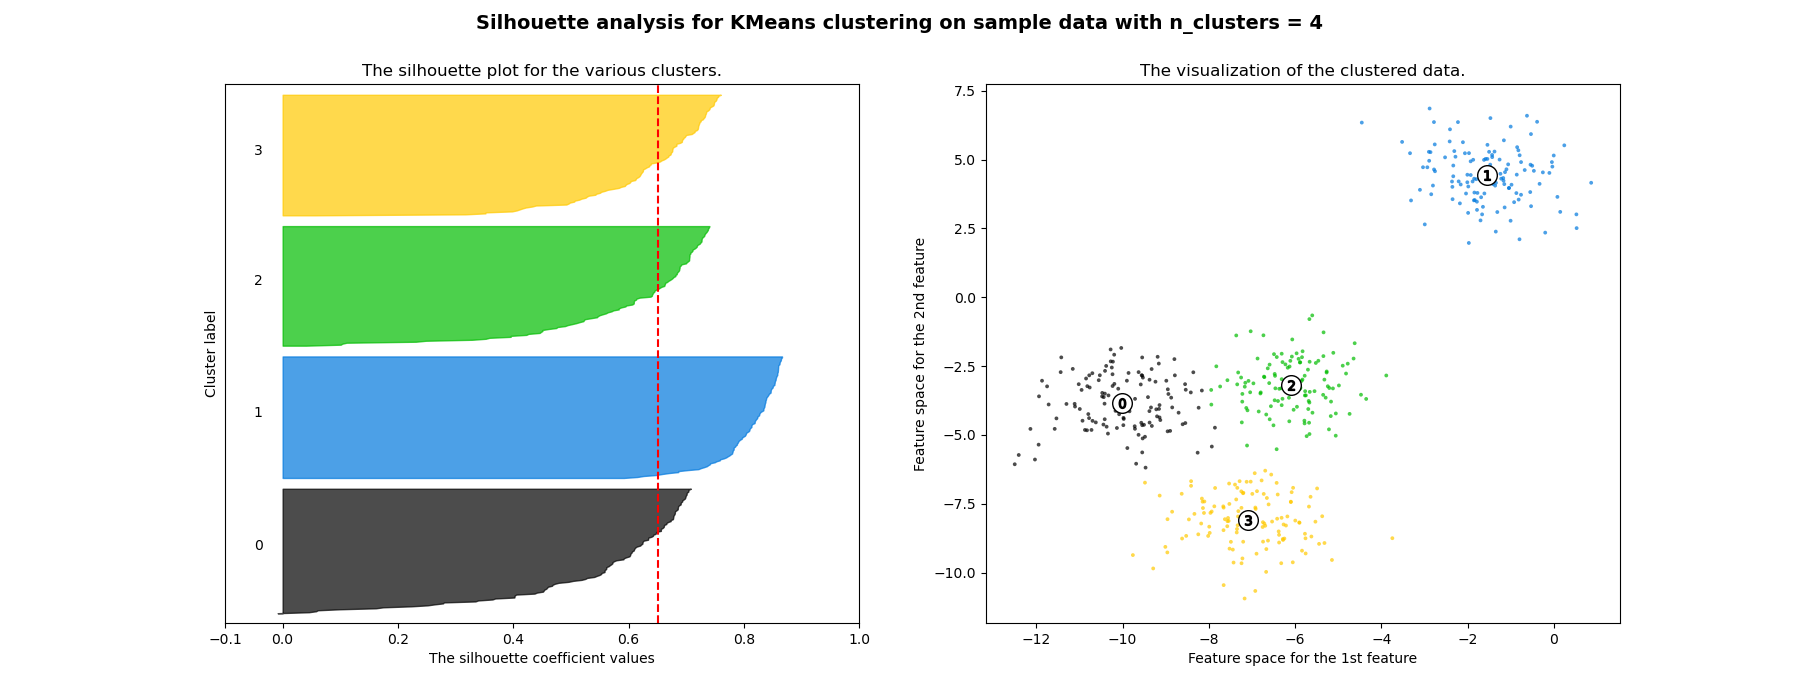
\includegraphics[width=.6\textwidth]{./figs/silouhette.png}
    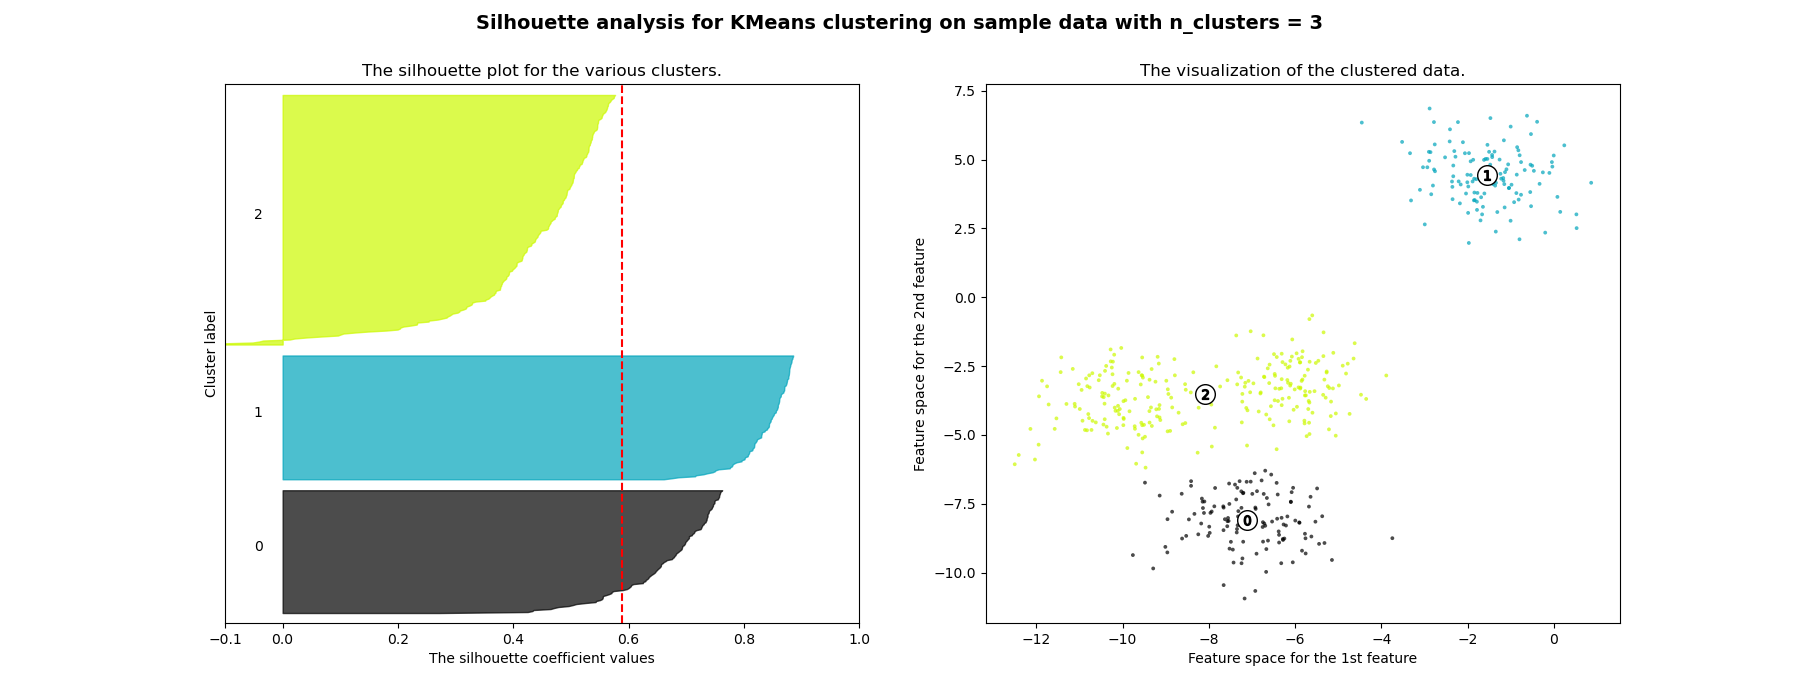
\includegraphics[width=.6\textwidth]{./figs/silouhette2.png}
    \caption{\tiny Figures from scikit-learn documentation}
    % \caption{\tiny Figures from \href{https://scikit-learn.org/stable/auto_examples/cluster/plot_kmeans_silhouette_analysis.html#sphx-glr-auto-examples-cluster-plot-kmeans-silhouette-analysis-py}{scikit-learn documentation}}
    \end{figure}
\end{frame}

\begin{frame}{K-means advantages and drawbacks}
\begin{columns}
\begin{column}{0.01\textwidth}
\begin{itemize}
    \item[] 
    \item[] 
    \item[] 
    \item[] 
\end{itemize}
\end{column}
    \column{0.3\linewidth}
        \textbf{Advantages}
        \begin{itemize}
            \item<1-> fast
            \item<2-> scales well
            \item<3-> converges well
            \item<4-> robust
        \end{itemize}
    \column{0.5\linewidth}
        \textbf{Drawbacks}
        \begin{itemize}
            \item<5-> \textbf{not suited for non-linear data}
            \item[\rightarrow]<6-> Density based clustering 
            \item[] 
            \item[] 
        \end{itemize}
    \column{0.2\linewidth}
    \includegraphics<5->[height=.8\textheight]{./figs/kmeans-non-linearity.png}
\end{columns}
\end{frame}

\subsection{HDBSCAN}
\begin{frame}{HDBSCAN}
    \centering
    \includegraphics<1>[width=.7\textwidth]{./figs/hdbscan/1.png}%
    \includegraphics<2>[width=.7\textwidth]{./figs/hdbscan/2.png}%
    \includegraphics<3>[width=.7\textwidth]{./figs/hdbscan/3.png}%
    \includegraphics<4>[width=.7\textwidth]{./figs/hdbscan/4.png}%
    \includegraphics<5>[width=.7\textwidth]{./figs/hdbscan/5.png}%
    \includegraphics<6>[width=.7\textwidth]{./figs/hdbscan/6.png}%
    \includegraphics<7>[width=.7\textwidth]{./figs/hdbscan/7.png}%
    \includegraphics<8>[width=.7\textwidth]{./figs/hdbscan/8.png}%
    \includegraphics<9>[width=.7\textwidth]{./figs/hdbscan/9.png}%
    \includegraphics<10>[width=.7\textwidth]{./figs/hdbscan/10.png}%
    \includegraphics<11>[width=.7\textwidth]{./figs/hdbscan/11.png}%
    \includegraphics<12>[width=.7\textwidth]{./figs/hdbscan/12.png}%
\end{frame}

\begin{frame}{A lot of options !}
    \centering
    \vspace{-.2cm}
    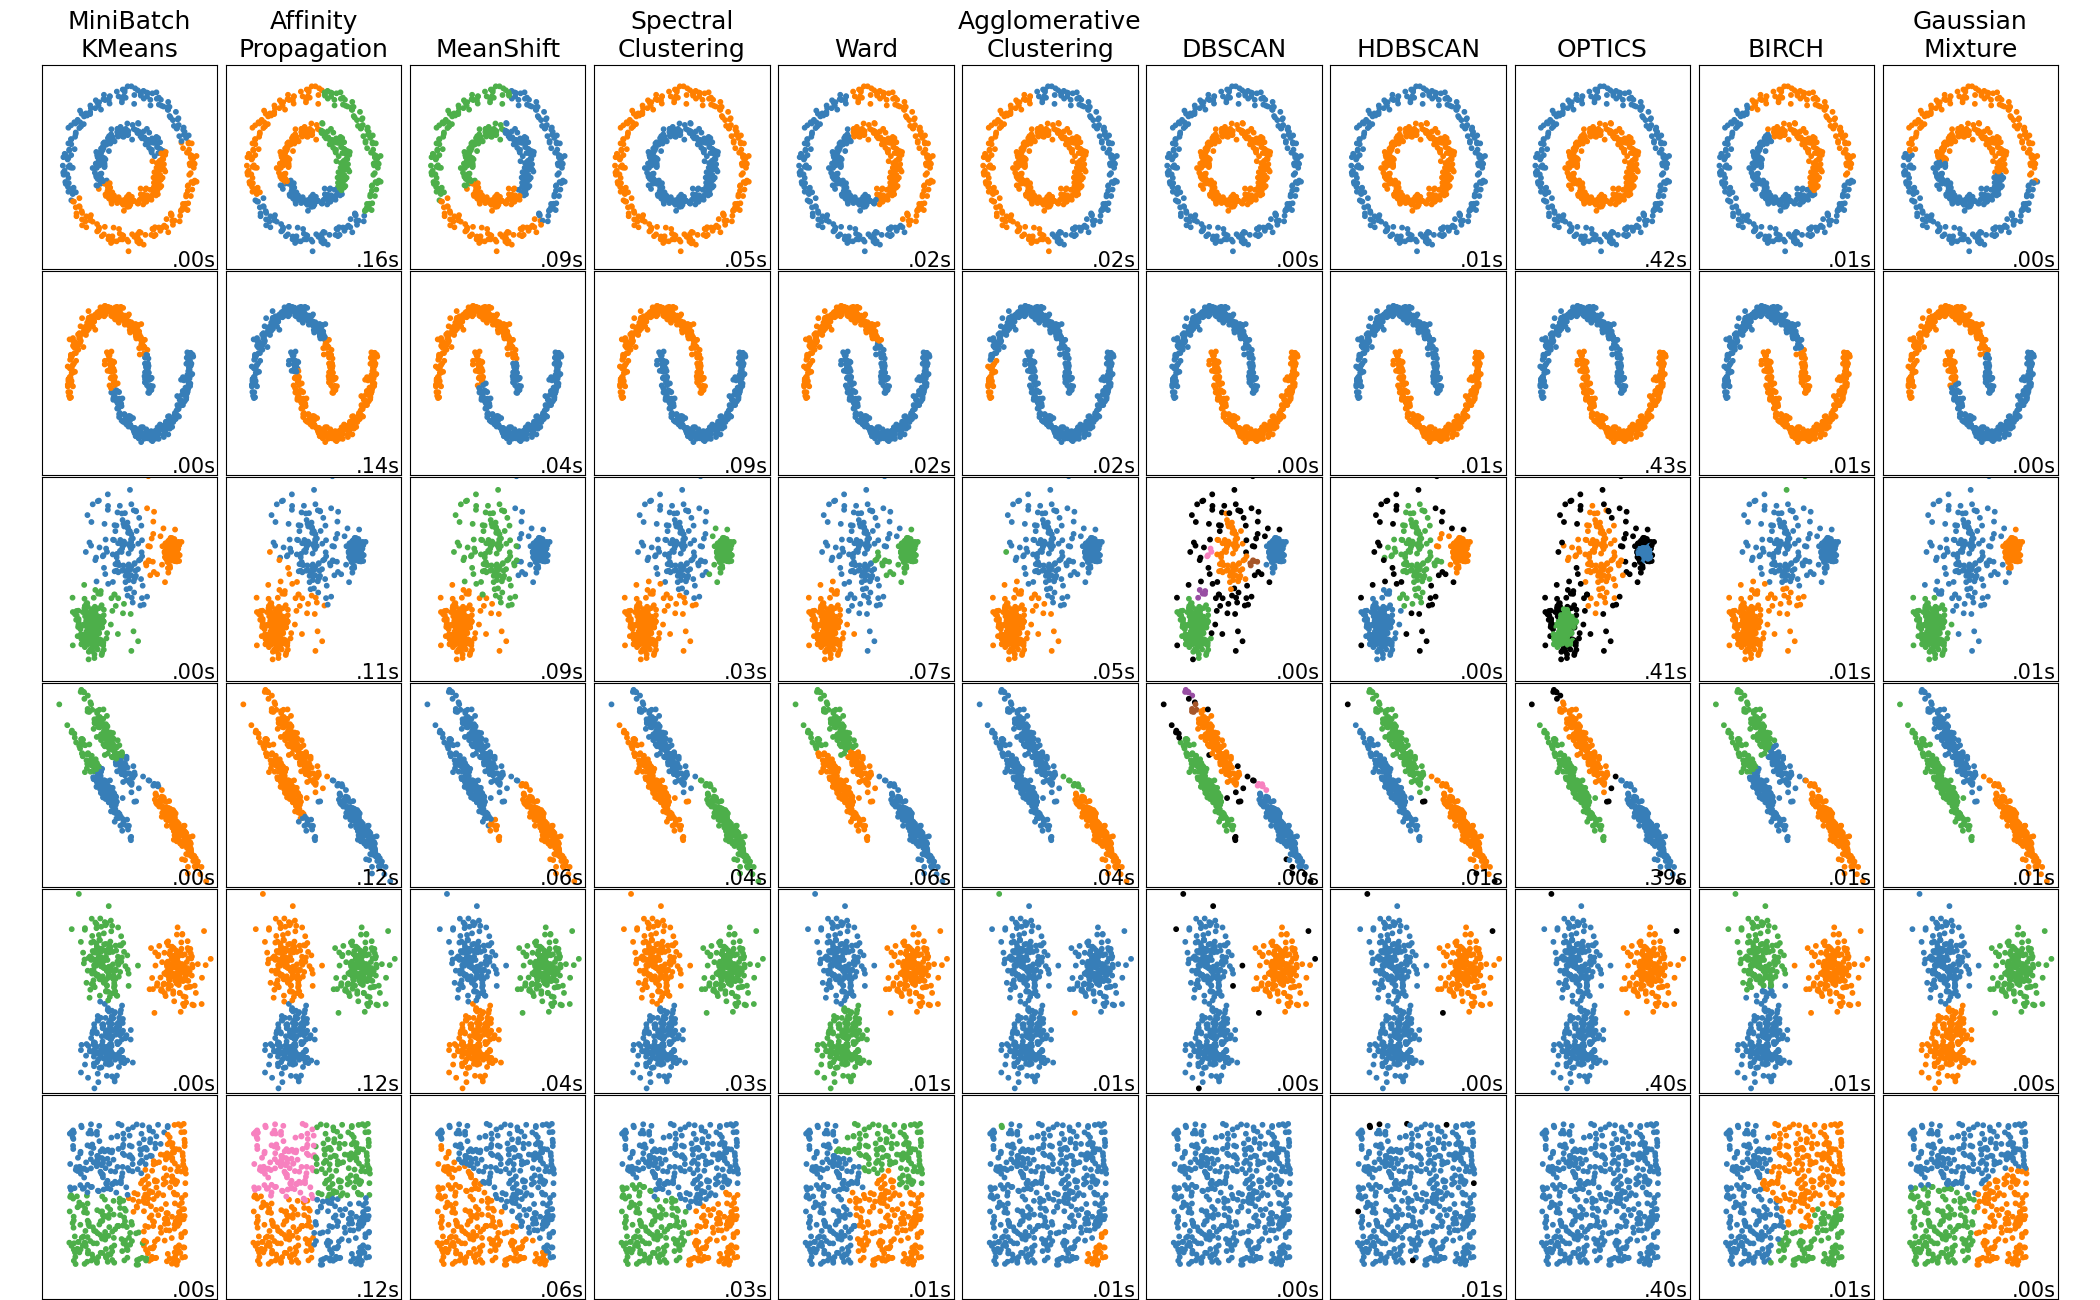
\includegraphics[width=.8\textwidth]{./figs/all_clusterings.png}
\end{frame}

\begin{frame}{Useful ressources}

\begin{itemize}
    \item \texttt{scikit-learn} docs !
    \item \href{https://www.youtube.com/@Deepia-ls2fo}{deepia}
    \item \href{https://www.youtube.com/@statquest}{StatQuest}
\end{itemize}
\end{frame}

\begin{frame}[plain]
    \Huge{\textbf{Thanks for you attention !}}
    
    \vfill
    
    \LARGE{\textbf{Let's practice !}}
\end{frame}

\appendix
% \printbibliography
% [heading=none]
\begin{frame}[allowframebreaks]{References}
\setbeamertemplate{bibliography item}{}
    {\footnotesize \printbibliography[heading=none]}
\end{frame}


\end{document}
